\documentclass[a4paper, fleqn]{article}
\usepackage[utf8]{inputenc}
\usepackage{amsmath}
\usepackage{amssymb}
\usepackage{caption}
\usepackage{mathtools}
\usepackage{amsfonts}
\usepackage{lastpage}
\usepackage{tikz}
\usepackage{float}
\usepackage{textcomp}
\usetikzlibrary{patterns}
\usepackage{pdfpages}
\usepackage{gauss}
\usepackage{fancyvrb}
\usepackage[table]{colortbl}
\usepackage{fancyhdr}
\usepackage{graphicx}
\usepackage{hyperref}
\usepackage[margin=2.5 cm]{geometry}

\setlength\parindent{0pt}
\setlength\mathindent{75pt}

\definecolor{listinggray}{gray}{0.9}
\usepackage{listings}
\lstset{
	language=,
	literate=
		{æ}{{\ae}}1
		{ø}{{\o}}1
		{å}{{\aa}}1
		{Æ}{{\AE}}1
		{Ø}{{\O}}1
		{Å}{{\AA}}1,
	backgroundcolor=\color{listinggray},
	tabsize=3,
	rulecolor=,
	basicstyle=\scriptsize,
	upquote=true,
	aboveskip={0.2\baselineskip},
	columns=fixed,
	showstringspaces=false,
	extendedchars=true,
	breaklines=true,
	prebreak =\raisebox{0ex}[0ex][0ex]{\ensuremath{\hookleftarrow}},
	frame=single,
	showtabs=false,
	showspaces=false,
	showlines=true,
	showstringspaces=false,
	identifierstyle=\ttfamily,
	keywordstyle=\color[rgb]{0,0,1},
	commentstyle=\color[rgb]{0.133,0.545,0.133},
	stringstyle=\color[rgb]{0.627,0.126,0.941},
  moredelim=**[is][\color{blue}]{@}{@},
}

\lstdefinestyle{base}{
  emptylines=1,
  breaklines=true,
  basicstyle=\ttfamily\color{black},
}

\def\checkmark{\tikz\fill[scale=0.4](0,.35) -- (.25,0) -- (1,.7) -- (.25,.15) -- cycle;}
\newcommand*\circled[1]{\tikz[baseline=(char.base)]{
            \node[shape=circle,draw,inner sep=2pt] (char) {#1};}}
\newcommand*\squared[1]{%
  \tikz[baseline=(R.base)]\node[draw,rectangle,inner sep=0.5pt](R) {#1};\!}
\newcommand{\comment}[1]{%
  \text{\phantom{(#1)}} \tag{#1}}
\def\A{\mathcal{A}}
\def\I{\mathcal{I}}
\def\E{\mathbb{E}}
\def\el{[\![}
\def\er{]\!]}
\def\dpip{|\!|}
\def\MeanN{\frac{1}{N}\sum^N_{n=1}}
\cfoot{Page \thepage\ of \pageref{LastPage}}
\DeclareGraphicsExtensions{.pdf,.png,.jpg}
\begin{document}
\section*{Reading}
\begin{itemize}
    \item Notes, section 1-3
\end{itemize}
\tableofcontents
\section{Intro}
\subsection{$k$-independence}
\begin{enumerate}
  \item For any distinct keys $x_0,...,x_k \in [u]\}$, the hash values $h(x_0),...,h(x_k)$ are independent random variables, that is, for any hash values $y_0,...,y_k \in [t]$ and $i \in [k], \Pr[h(x_i)=y_i] = \Pr[h(x_i) = y_i | \bigwedge_{j\in[k]\\\{i\}} h(x_j) = y_j]$.
  \item For any $x \in [u]$, $h(x)$ is uniformly distributed in $[t]$.
\end{enumerate}
\subsection{Example of linear probing}
\begin{verbatim}
h(a) = 2, h(b) = 3, h(c) = 2, h(d) = 3
|1|2|3|4|5|6|
| |a| | | | |
| |a|b| | | |
| |a|b|c| | |
| |a|b|c|d| |
c?, h(c) = 2
| |a|b|c|d| |
   ^ ^ ^
-a, h(a) = 2
| |a|b|c|d| |
| | |b|c|d| |
| |c|b| |d| |
| |c|b|d| | |
\end{verbatim}
\section{Linear probing with 5-independence}
A run $R$ is a the longest consecutively amount of filled positions. When proving we talk about something called dyadic intervals, a dyadic $l$-interval is an interval of length $2^l$, containing positions $[i2^l,(i+1)2^l)$ where $i \in [t/2^l]$. An interval is near-full if at least $3/4 2^l$ keys from $S/\{q\}$ hash into it.
\subsection{Lemma 2}
Consider a run $R$ of length $r \geq 2^{l+2}$. Then one of the first four $l$-intervals intersecting $R$ must be near full.
\paragraph{Proof}
\begin{center}
  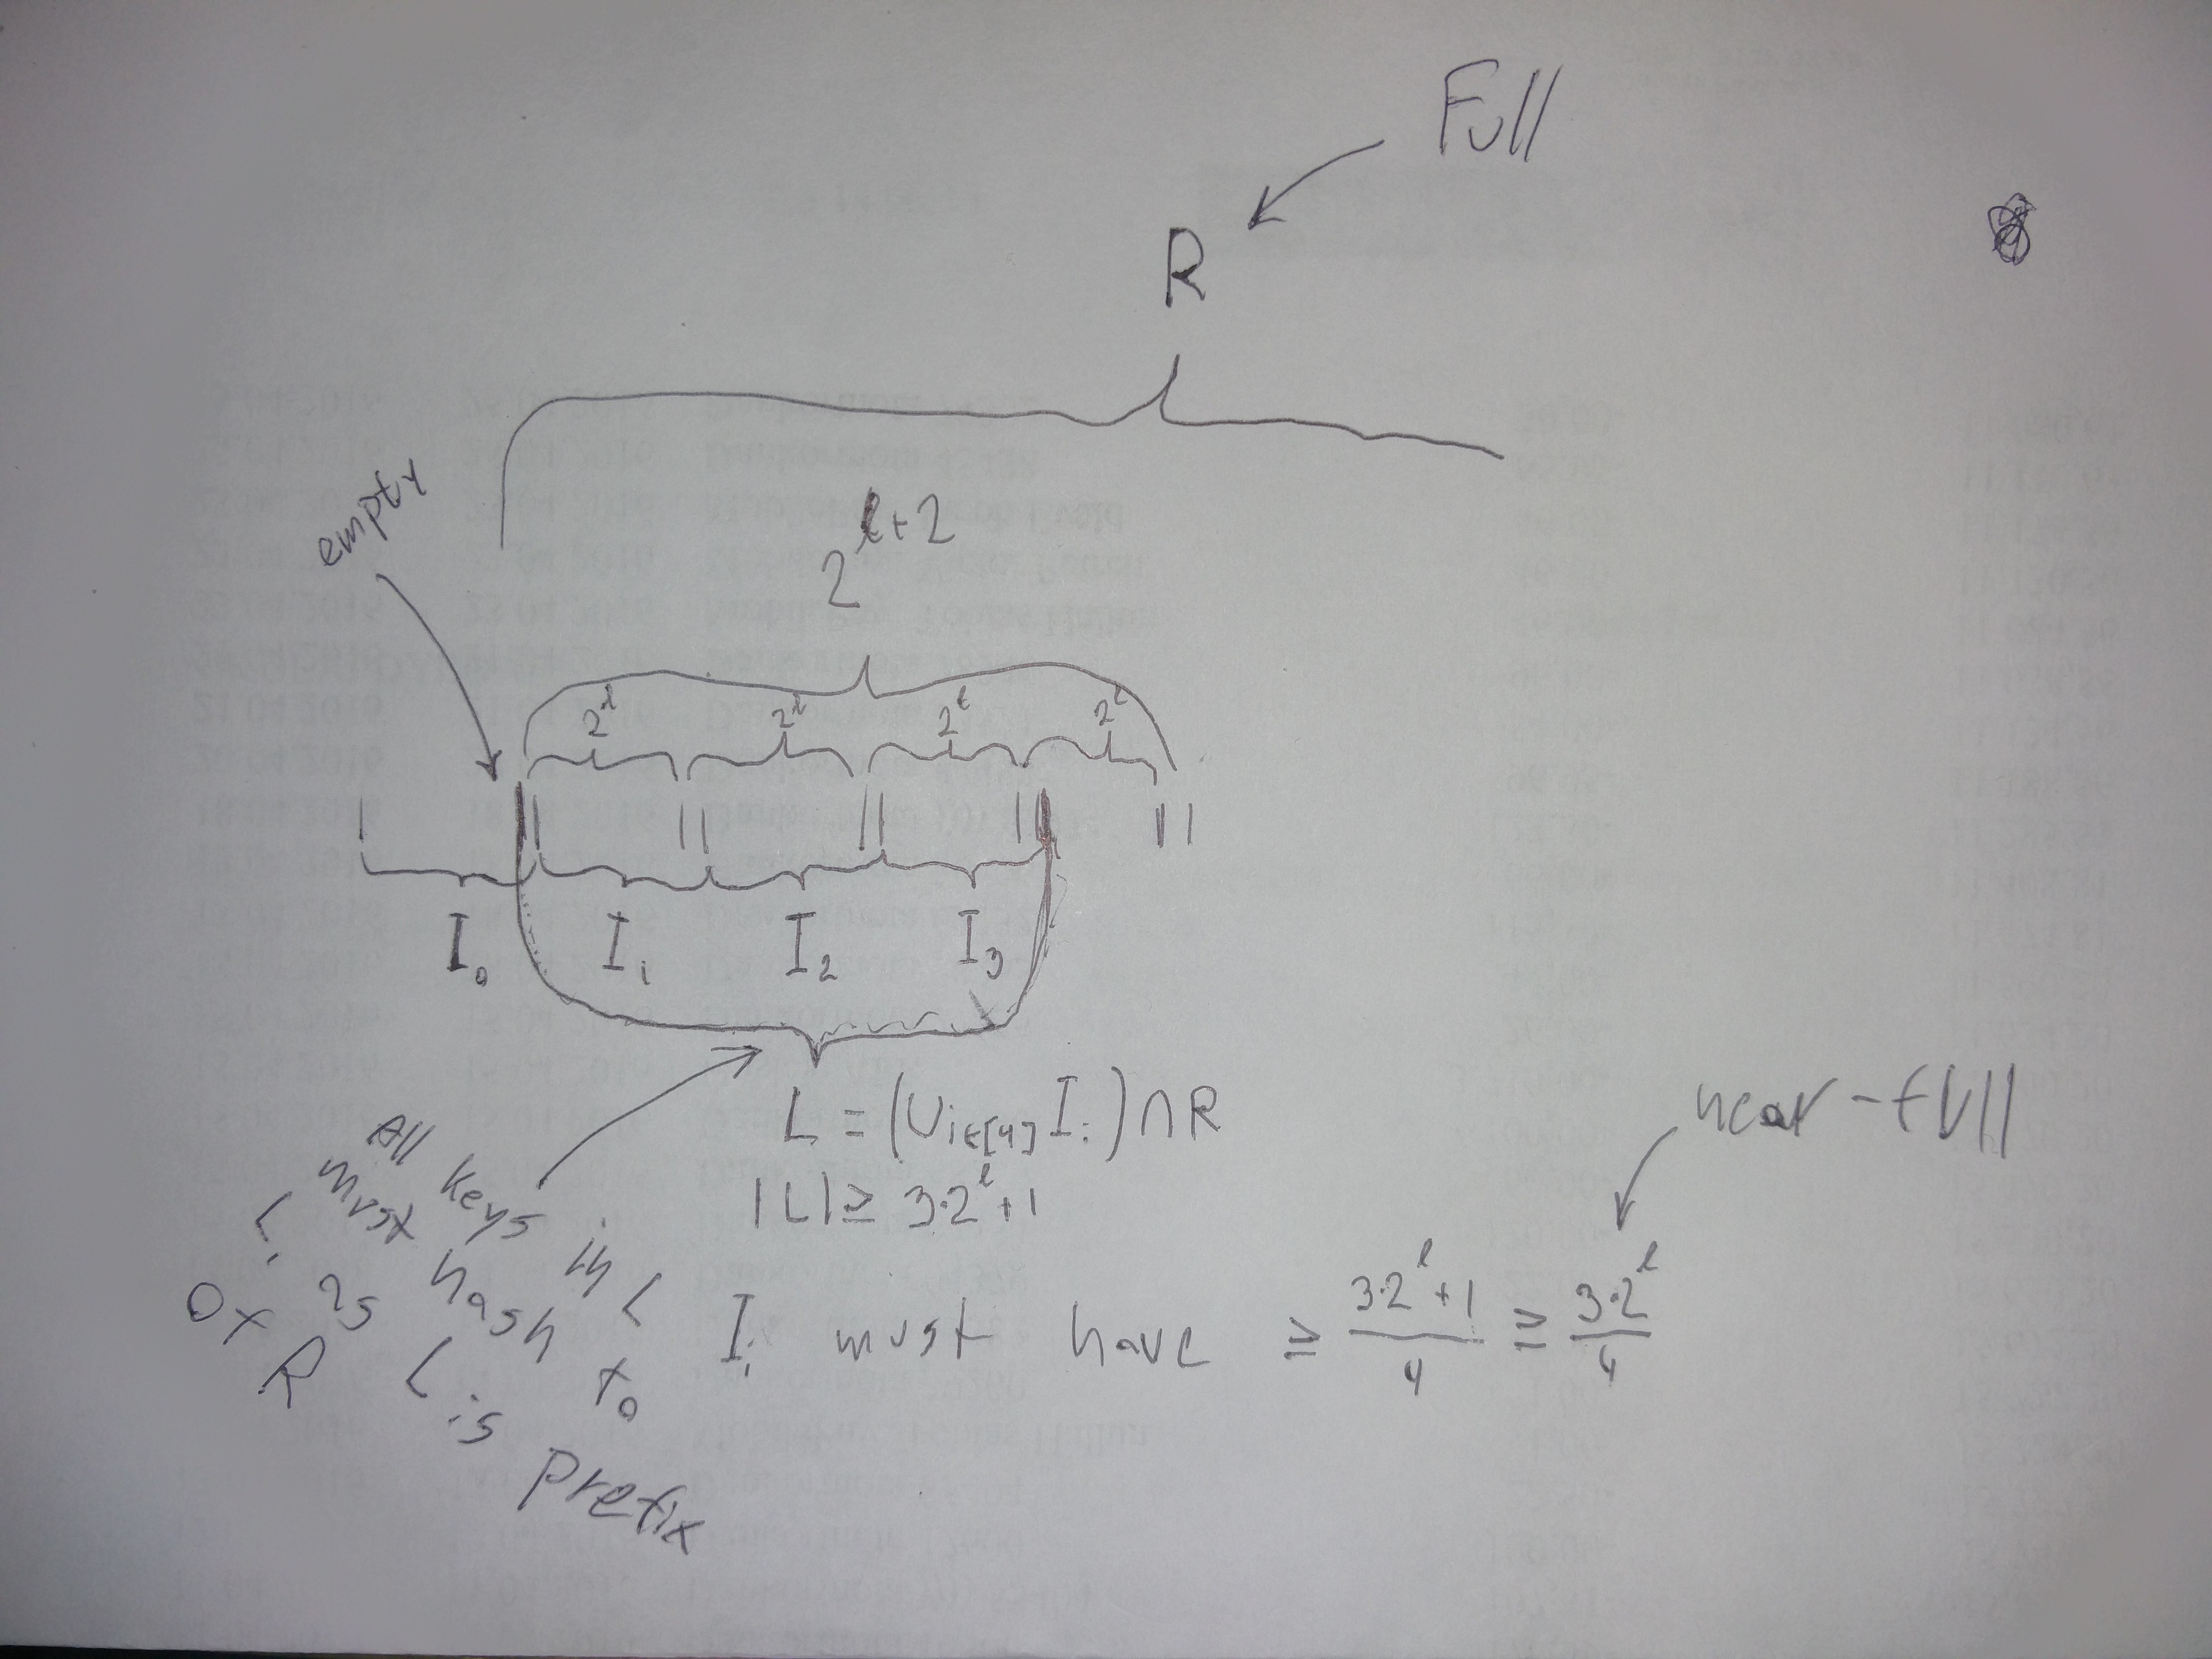
\includegraphics[width=\textwidth]{./fig_1_8_linearProbing.jpg}
\end{center}
\subsection{Lemma 3}

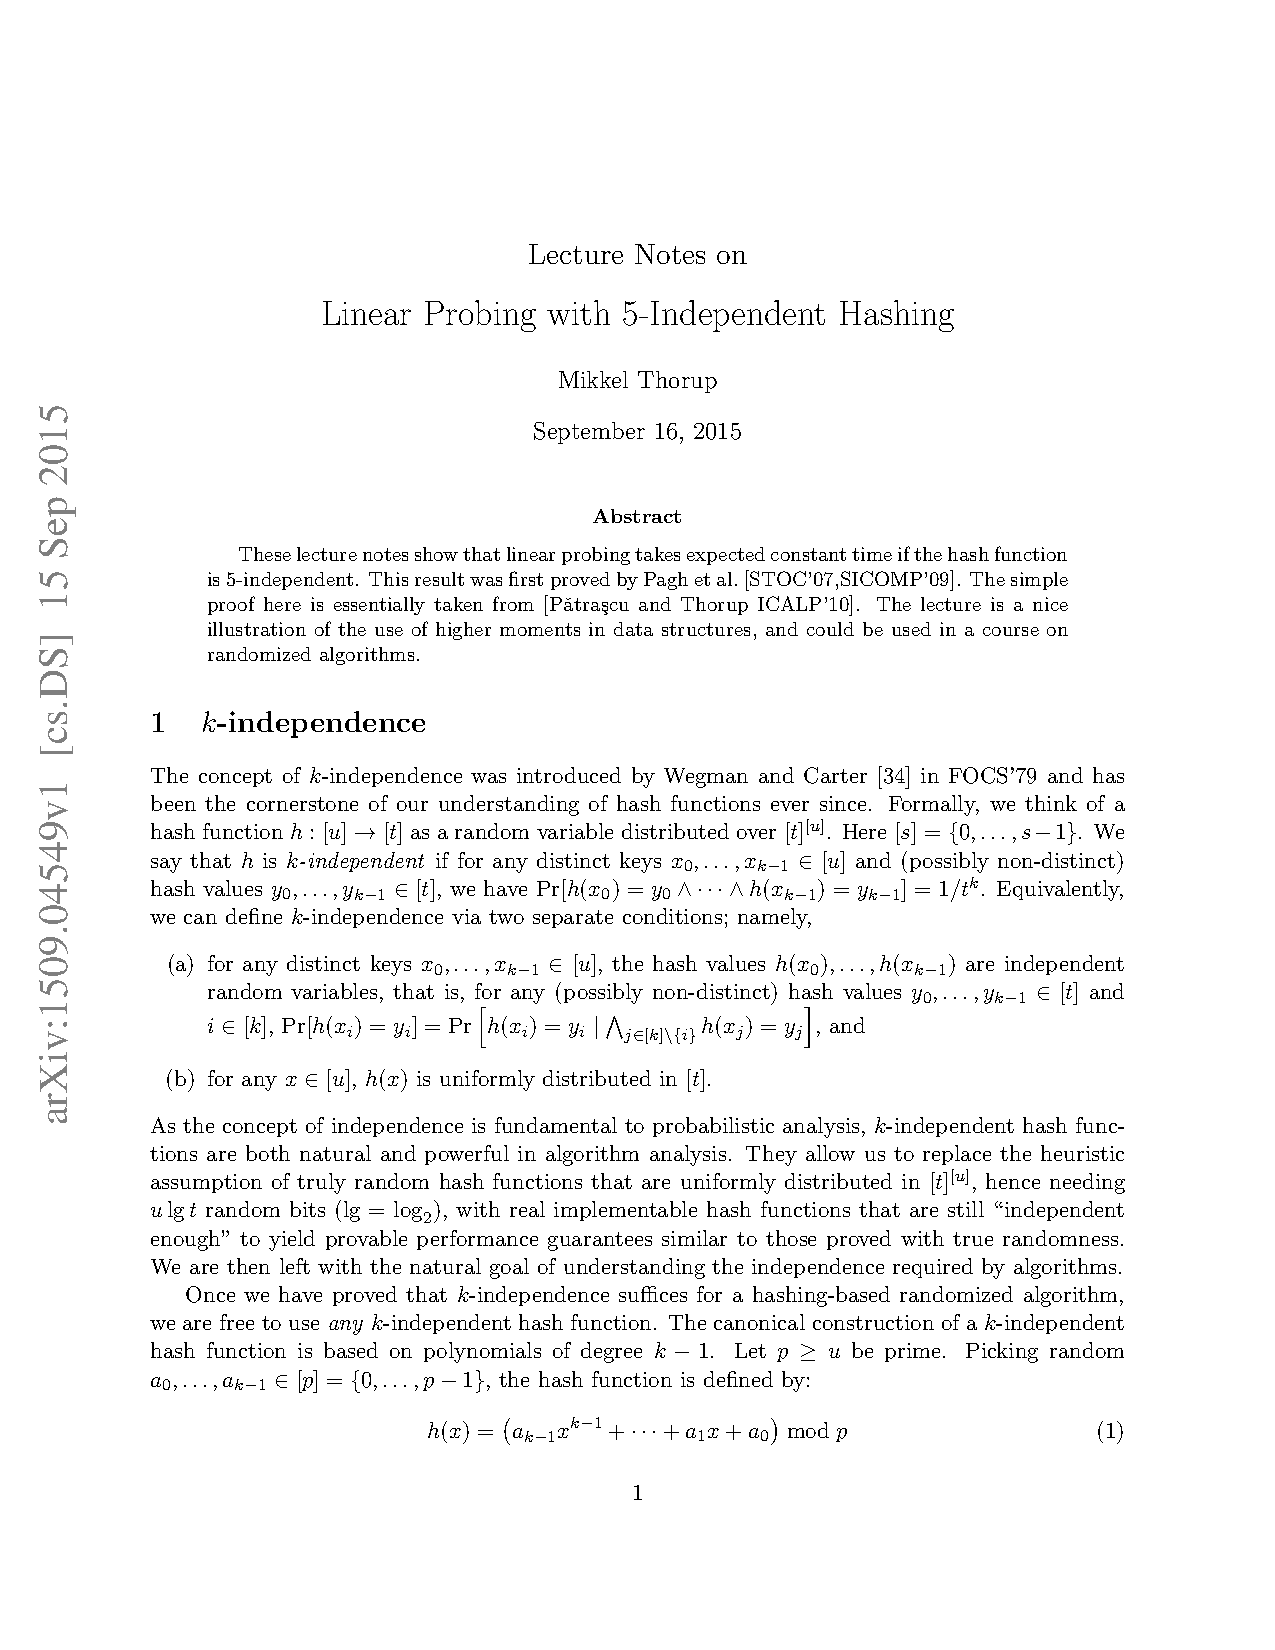
\includepdf[pages=-]{./notes_8_linearProbing.pdf}
\end{document}
